%!TEX root = project.tex

\chapter{Methodology}

For the project we used the waterfall methodology. We started by mapping out the requirements for the project. Then we designed how the UI would be implemented, how the user should be able to add an account on the system.  We used GitHub for source control of the program, we also used overleaf for collaboration with the dissertation. 

\section{Requirements}

We mapped out the requirements of our project:
\begin{itemize}
\item We would need a server or some form of central point that connects the users to any back-end that we \item would require too run the game.
\item We decided the system required a login system that would allow a user to create an account or login to an existing one.
\item We then would need a system that allowed players to connect to other users.
\item We would need a lobby systems where players can wait for a game to start or wait for other players to join the game.
\item Once the game has ended we would need a system that could keep track of the players games and achievements such as a scoreboard system.
\item The separate systems speak to the client and do not need to send data to each other, this will allow the system to be interchangeable.
\item Element of the system should be capable of being replaced by another system, without replacing other parts of the system. For example, if we decided to change the database or language for the scoreboard system, we should be able to do so without having to change any part of the login system, the match making system and minimal changes to the game itself, if any.
\end{itemize}


The game Itself:
\begin{itemize}
\item Must have a procedural track to allow for non repetitive play.
\item Different versions of the game should connect to any instance and should not need to specify whether they can play with desktop or virtual reality headset users.
\item Desktop platforms must be able to see head and hand movement from the head mount display players.
\item Players must start in specified positions and must not have to enter any input for this to occur.
\item The Races must have a start and end point.
\end{itemize}

\newpage
\section{Design Stage}

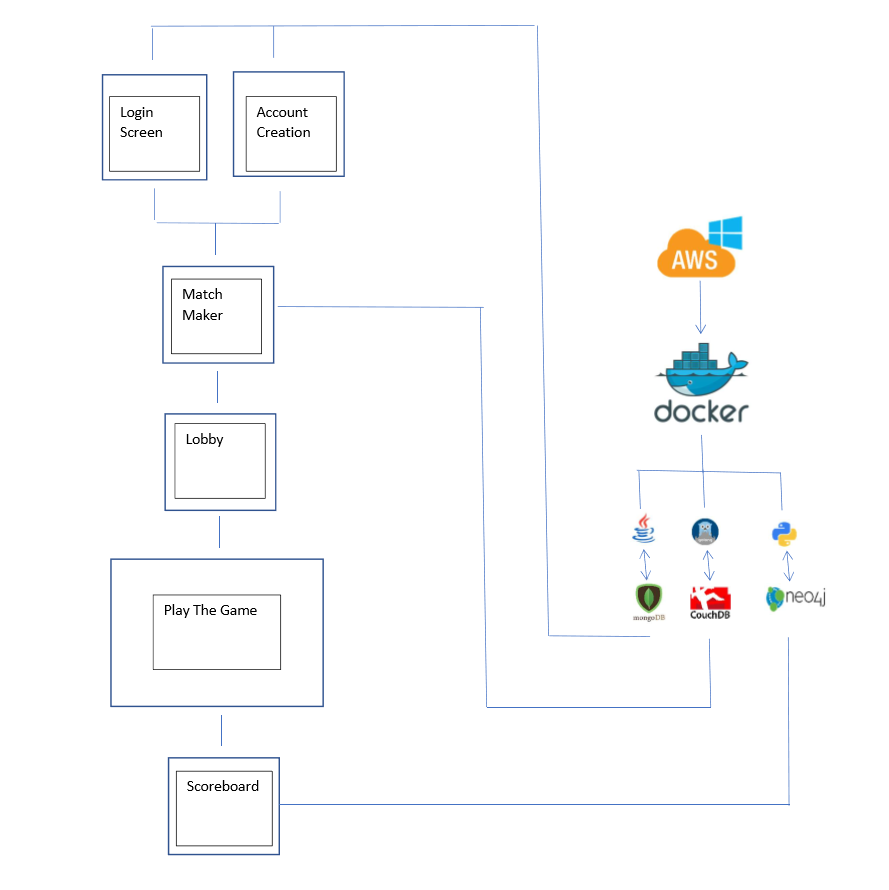
\includegraphics[width=1\columnwidth]{img/Overview.PNG}

During the design stage, we had to map out the system and decide on which elements were needed and how they could be implemented. From the very start we knew that the game itself must be implemented in either Unity with C\# or using the Unreal 4 engine with C\+\+. Our knowledge and experience of the unreal engine and with any of the C++ language is very limited, were as we already have a working knowledge of unity and C\#. So we went with Unity. Using any form of third gaming engine would not be practical as the libraries for the virtual reality devices have been focuses on these two implementations.\newline

Our login system

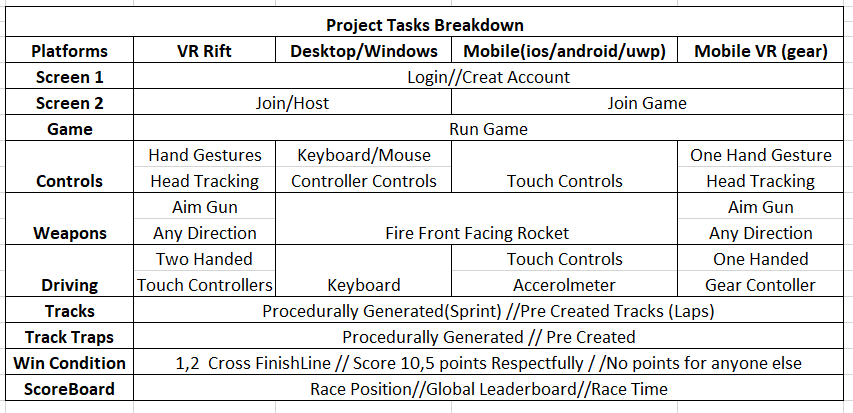
\includegraphics[width=1\columnwidth]{img/breakdown.PNG}

Our match making system

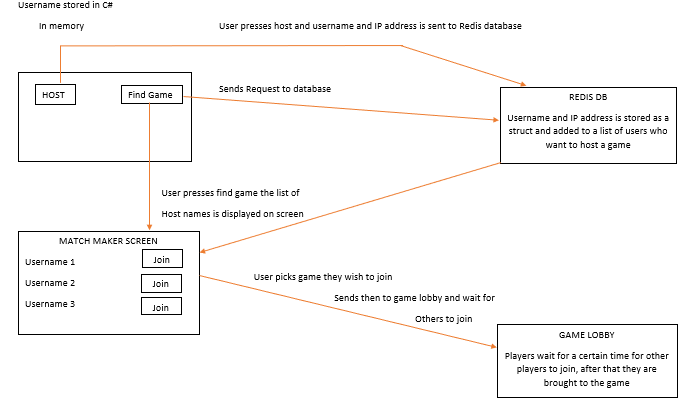
\includegraphics[width=1\columnwidth]{img/redisMatch.PNG}

An overview of the game

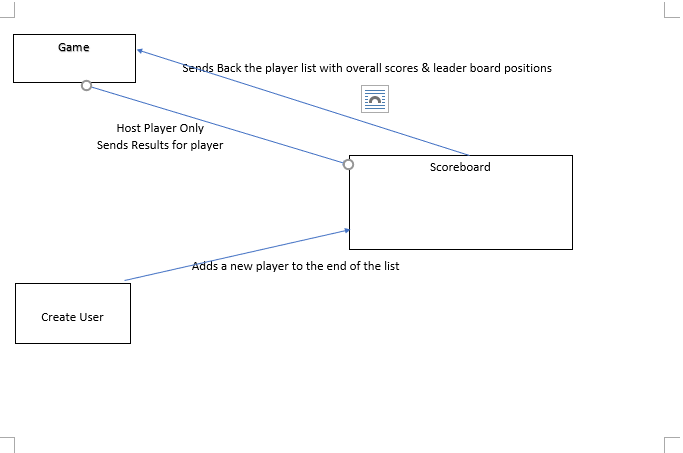
\includegraphics[width=1\columnwidth]{img/MariaDBPic.PNG}

An overview of our scoreboard system

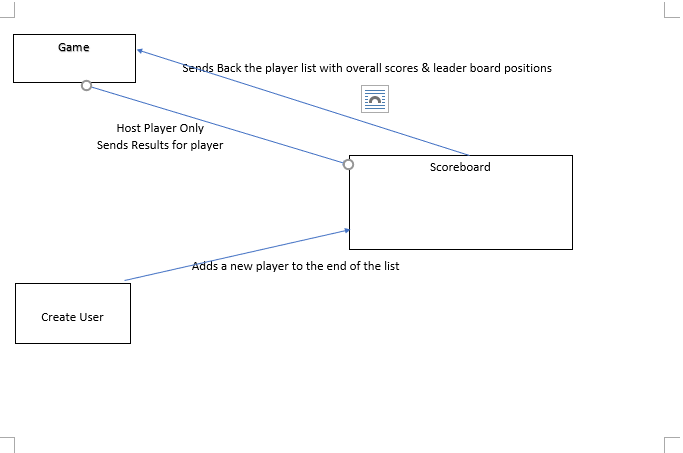
\includegraphics[width=1\columnwidth]{img/MariaDBPic.PNG}

\newpage
\section{Implementation}

\newpage
\section{Integration and System Testing}